\subs{Cosformer}
\label{subsec:cosformer}
\subsubs{Softmax的两个关键属性}
CosFormer\cite{zhen2022cosformer}经验性地确定了softmax操作的两个关键属性,这些属性对其性能可能起到重要作用:
1)它确保注意力矩阵$A$中的所有值都是非负的;
2)它提供了一个非线性重新加权机制,用于集中注意力连接的分布并稳定训练\cite{titsias2016one}。

基于上述性质,Cosformer完全放弃了 softmax 归一化,同时仍然具有非负性和重新加权机制。它包含两个主要组件:线性投影内核 $\phi_{linear}$ 和基于 cos 的重新加权机制。

\subsubs{线性投影内核$\phi_{\text{linear}}$}
回顾注意力的一般形式
\begin{equation}
   \mathcal{O} = \mathcal{A}(x) = \left[\mathcal{O}_1,\hdots, \mathcal{O}_N \right]^T, \quad \mathcal{O}_i
 = \sum_j \frac{\mathcal{S}(Q_i,K_j)}{\sum_j \mathcal{S}(Q_i,K_j)}V_j,
\end{equation}
定义线性相似度为:
\begin{equation}
\mathcal{S}(Q,K)=\mathrm{s}(\phi_{\text{linear}}(Q),\phi_{\text{linear}}(K))=\mathrm{s}(Q',K')
\label{eq:qk}
\end{equation}
其中$\phi_{\text{linear}}$是将查询$Q$和键$K$映射到我们所需表示$Q'$和$K'$的转换函数,
$\mathrm{s}$是一个可以线性分解的函数,用于衡量$Q'$和$K'$之间的相似性。
具体而言,为了确保完全正的注意力矩阵$A$并避免聚集负相关信息,我们采用$\mathrm{ReLU}(\cdot)$作为转换函数,从而有效消除负值:
\begin{equation}
\textstyle{
\phi_{\text{linear}}(x) = \mathrm{ReLU}(x)
}
\end{equation}
由于$Q'$和$K'$只包含非负值,可以直接计算它们的点积$s(x,y) =xy^T, x,y\in \mathbb R^{1\times d}$,然后进行逐行归一化以计算注意力矩阵:
\begin{equation}
\textstyle{
\mathcal{O}i = \frac{\sum^{N}{j=1}f(\phi_{\text{linear}} (Q_i), \phi_{\text{linear}}({K_j})) V_j}{\sum^{N}{j=1}f(\phi{\text{linear}} (Q_i), \phi_{\text{linear}}({K_j}))} = \frac{\sum^{N}{j=1}(\mathrm{ReLU} (Q_i) \mathrm{ReLU}({K_j})^T) V_j}{\sum^{N}{j=1}(\mathrm{ReLU} (Q_i) \mathrm{ReLU}({K_j})^T)}
}
\end{equation}

基于公式
\begin{equation}
\textstyle{
    O_i = \frac{\sum^{N}_{j=1}(\phi (Q_i) \phi({K_j})^T) V_j}{\sum^{N}_{j=1}(\phi (Q_i) \phi({K_j})^T)}.
\label{eq: rewrite att},
}\end{equation}
重新排列点积的顺序,得到以线性复杂度表示的提出的注意力公式:
\begin{equation}
\textstyle{
\label{eq: relu attention}
\mathcal{O}i = \frac{\mathrm{ReLU} (Q_i) \sum^{N}{j=1}\mathrm{ReLU}({K_j})^T V_j}{\mathrm{ReLU} (Q_i)\sum^{N}_{j=1} \mathrm{ReLU}({K_j})^T}
}
\end{equation}

\vspace{-2mm}

\subsubs{基于余弦的重加权机制}
\cite{titsias2016one, gao2017properties} 指出,通过 softmax attention 引入的非线性重新加权机制,可以集中注意力权重的分布,从而稳定训练过程。\cite{zhen2022cosformer}还通过实验证明,这种机制可以惩罚远距离连接并在某些情况下强制局部性。事实上,这种局部性偏差,即大部分上下文依赖关系来自相邻的标记,在下游自然语言处理任务中普遍观察到~\cite{clark2019does, kovaleva2019revealing},如图~\ref{fig: reweight}~(1)所示。

基于上述假设,还需要实现 softmax 的第二个性质,即一种可分解的重新加权机制,能够向注意力矩阵引入最近性偏差。因此,Cosformer提出了一种基于余弦的重新加权机制,因为它完全符合上述目的:1)Ptolemy 定理确保了余弦权重可以分解为两个求和项;2)如图~\ref{fig: reweight}(4)所示,余弦函数在相邻的标记上放置更多的权重,从而强制实现局部性。另外,通过比较图\ref{fig: reweight}~(2)和(3)中的注意力矩阵,可以发现相较于没有重新加权机制的情况,Cosformer更加强调局部性。

\begin{figure}[t]
   \begin{center}
   {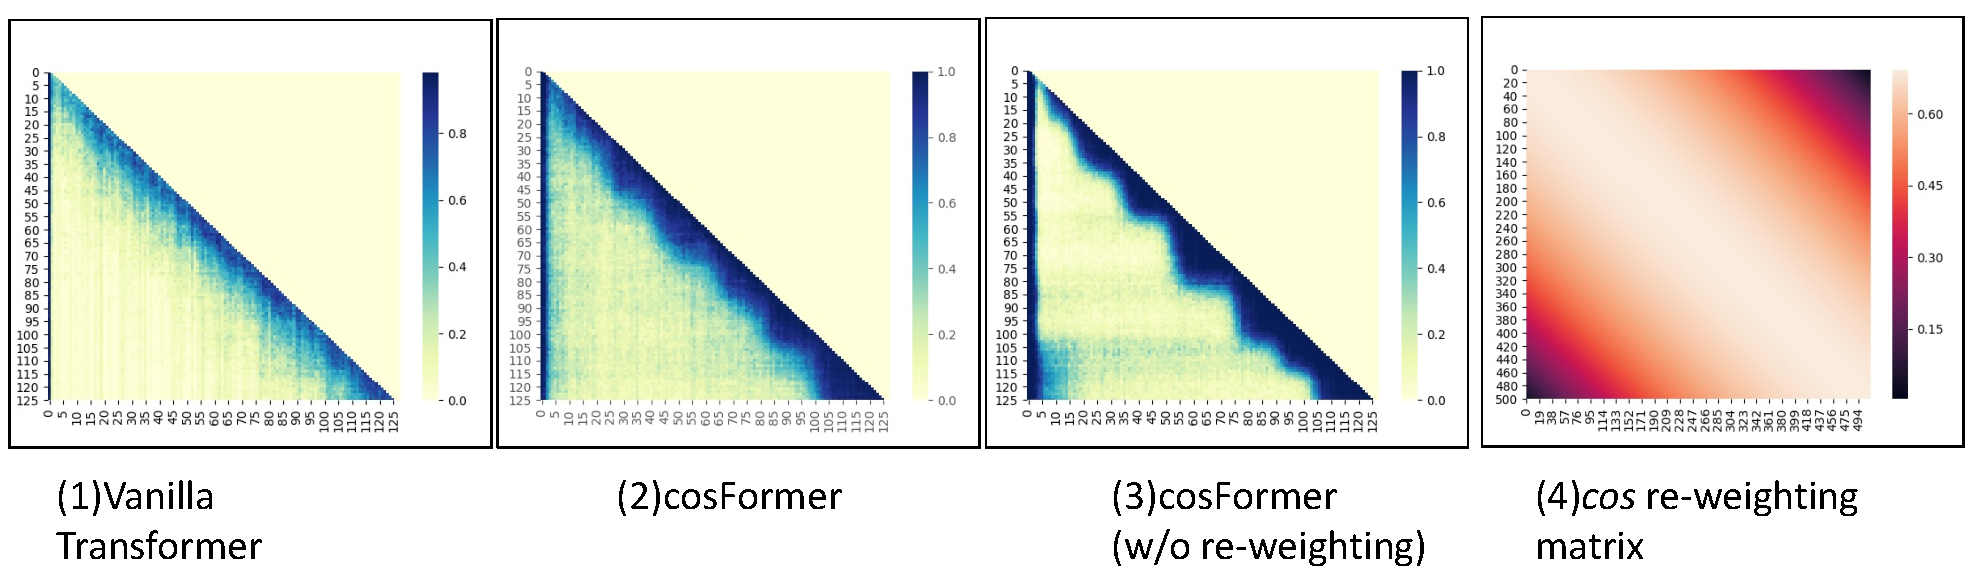
\includegraphics[width=1\linewidth]{figs/cosformer/reweight.pdf}} 
   \vspace{-8mm}
   \end{center}
\caption{(1): Vanilla Transformer的注意力矩阵。(2): Cosformer 的注意力矩阵。(3): 没有重新加权机制的 Cosformer 的注意力矩阵。(4): 基于余弦距离的矩阵可视化。在重新加权后,我们可以看到注意力矩阵的对角区域具有更平滑的注意力分布,呈现出类似于Vanilla Transformer的模式,有助于稳定训练。摘自~\cite{zhen2022cosformer}}
\vspace{-2mm}
   \label{fig: reweight}
\end{figure}

具体而言,结合~\eqref{eq:qk},带有余弦重新加权的模型定义为:
\begin{equation}
\textstyle{
s(Q_i^{'}, K_j^{'})
= Q_{i}^{'}K_{j}^{'T}\cos\left(\frac{\pi}{2} \times \frac{i-j}{M} \right)
}
\end{equation}
\cite{zhen2022cosformer}利用 Ptolemy 定理将这个公式分解为:
\scriptsize
\begin{equation}
\begin{aligned}
Q_{i}^{'}K_{j}^{'T}\cos\left(\frac{\pi}{2} \times \frac{i-j}{M} \right) 
&=Q_{i}^{'}K_{j}^{'T}\left(\cos\left(\frac{\pi i}{2M}\right)\cos\left(\frac{\pi j}{2M}\right) + \sin\left(\frac{\pi i}{2M}\right)\sin\left(\frac{\pi j}{2M}\right)\right)\ \\
&= \left(Q_{i}^{'} \cos \left(\frac{\pi i}{2M}\right)\right)\left(K_{j}^{'}\cos\left(\frac{\pi j}{2M}\right)\right)^{T} + \left(Q_{i}^{'}\sin\left(\frac{\pi i}{2M}\right)\right)\left(K_{j}^{'} \sin\left(\frac{\pi j}{2M}\right)\right)^{T}
\end{aligned}
\end{equation}
\normalsize

其中,$\small{i ,j= 1,...,N, M \geq N}$,$\small{Q^{'} = \mathrm{ReLU}(Q),K^{'} = \mathrm{ReLU}(K)}$。
令 $\small{Q_{i}^{\cos} =Q_{i}^{'} \cos \left(\frac{\pi i}{2M}\right)}$,$\small{Q_{i}^{\sin} =Q_{i}^{'} \sin \left(\frac{\pi i}{2M}\right)}$,

$\small{K_j^{\cos} =K_{j}^{'}\cos\left(\frac{\pi j}{2M}\right)}$,$\small{K_j^{\sin} =K_{j}^{'}\sin\left(\frac{\pi j}{2M}\right)}$,
则提出的注意力模块的输出可以表示为:
\begin{equation}
\label{eq appendix}
\textstyle{
O_i = \frac{\sum_{j=1}^N f(Q_i^{'}, K_j^{'}) V_j}{\sum^{N}{j=1} f(Q_i^{'}, K_j^{'}) }
= \frac{\sum{j=1}^N Q_{i}^{\cos} \left( \left( K_j^{\cos} \right)^TV_j \right)+\sum_{j=1}^N Q_{i}^{\sin} \left(\left( K_j^{\sin} \right)^T V_j \right)}{\sum_{j=1}^N Q_{i}^{\cos} \left( K_j^{\cos} \right)^T+\sum_{j=1}^N Q_{i}^{\sin} \left( K_j^{\sin} \right)^T },
}
\end{equation}

其中 $O_i$ 是注意力模块输出的序列中第 $i$ 个位置的值。
不失一般性,Cosformer的时间复杂度是线性的,表示为:
\begin{equation}
\textstyle{
\mathcal{O} = \mathcal{S}(Q, K)V
=(Q^{\cos}K^{\cos} + Q^{\sin}K^{\sin})V
=Q^{\cos}(K^{\cos}V) + Q^{\sin}(K^{\sin}V)
}
\end{equation}

从位置编码的角度来看, Cosformer 可以看作是一种将相对位置偏差引入高效Transformer的新方法。